Das Docker Compose Setup von LearnHub besteht aus zwei separaten 
Compose Files. Das erste definiert die eigentliche Anwendung mit 
allen Services, das zweite läuft als eigenständiger Stack und 
betreibt Traefik als Reverse-Proxy. Durch diese Trennung kann 
Traefik unabhängig von der Anwendung aktualisiert oder neugestartet 
werden.

\subsubsection{Traefik Stack}

Traefik läuft in einem eigenen Compose Stack und erstellt dabei 
auch das externe Docker-Netzwerk \texttt{learnhubnet}, über das 
alle Services miteinander kommunizieren. Abbildung~\ref{fig:compose-traefik} 
zeigt das Traefik Compose File.

\begin{figure}[H]
    \centering
    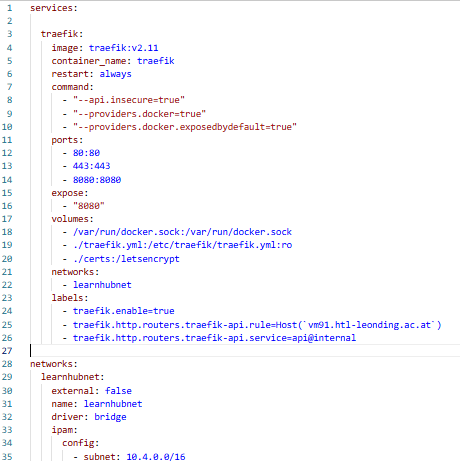
\includegraphics[width=0.9\textwidth]{pics/traefik_learnhub.png}
    \caption{Docker Compose File für Traefik}
    \label{fig:compose-traefik}
\end{figure}

Wie in Abbildung~\ref{fig:compose-traefik} zu sehen, ist Traefik 
der einzige Service der Ports nach außen öffnet, nämlich Port 80 
für HTTP und Port 443 für HTTPS. Zusätzlich ist Port 8080 für 
das Traefik-Dashboard geöffnet. Alle anderen Services sind von 
außen nicht direkt erreichbar. Das Netzwerk \texttt{learnhubnet} 
wird hier mit dem Subnetz \texttt{10.4.0.0/16} angelegt und als 
externes Netzwerk markiert, damit andere Compose Stacks es 
einbinden können. Traefik erkennt automatisch welche Services 
gestartet werden, indem der Docker-Socket 
\texttt{/var/run/docker.sock} in den Container gemountet wird. 
Dadurch kann Traefik die laufenden Container beobachten und deren 
Routing-Regeln aus den Labels lesen. Zusätzlich wird eine 
\texttt{traefik.yml} Konfigurationsdatei eingebunden sowie ein 
\texttt{certs} Ordner für SSL-Zertifikate.

\subsubsection{LearnHub Stack}

Das LearnHub Compose File definiert vier Services: Frontend, 
Backend, MySQL und einen Nginx-Upload-Server. 
Abbildung~\ref{fig:compose-learnhub} zeigt das vollständige 
Compose File.

\begin{figure}[H]
    \centering
    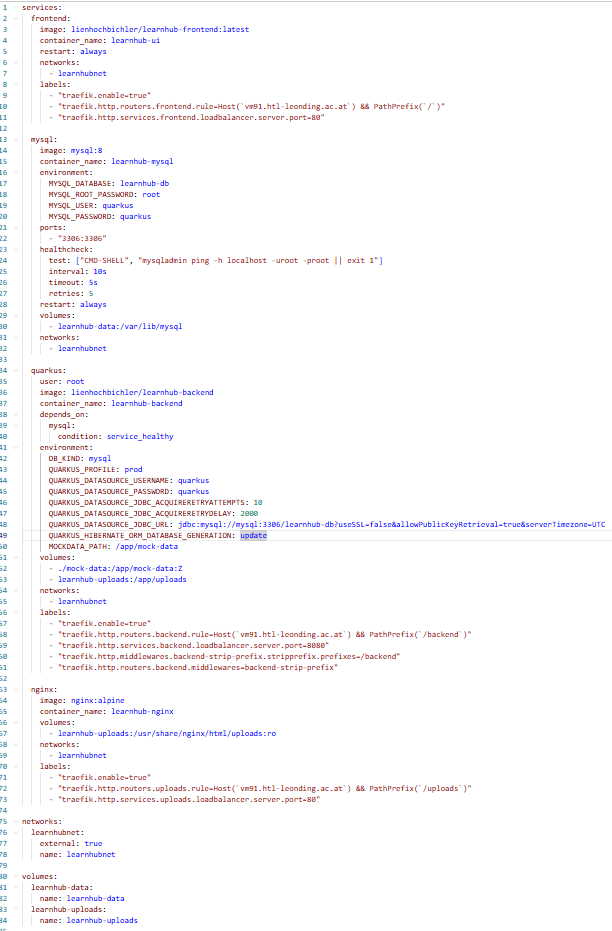
\includegraphics[width=0.9\textwidth]{pics/compose_learnhub.png}
    \caption{Docker Compose File von LearnHub}
    \label{fig:compose-learnhub}
\end{figure}

Wie in Abbildung~\ref{fig:compose-learnhub} zu sehen, verwendet 
jeder Service das entsprechende Docker-Image von Docker Hub. Das 
Frontend verwendet \texttt{lienhochbichler/learnhub-frontend} und 
das Backend \texttt{lienhochbichler/learnhub-backend}. Beide sind 
mit \texttt{restart: always} konfiguriert, was bedeutet dass sie 
bei einem Absturz oder Neustart der VM automatisch wieder 
hochfahren.

Jeder Service trägt seine Routing-Regeln als Labels direkt bei 
sich. Das Frontend ist unter dem Root-Pfad \texttt{/} erreichbar, 
das Backend unter \texttt{/backend} und die hochgeladenen Dateien 
unter \texttt{/uploads}. Für das Backend gibt es zusätzlich eine 
Middleware die den Prefix \texttt{/backend} aus der URL entfernt 
bevor die Anfrage den Container erreicht, da Quarkus intern keine 
Pfadpräfixe erwartet. Das Backend bekommt außerdem mehrere 
Umgebungsvariablen mitgegeben, darunter die Datenbankverbindung 
mit dem internen Hostnamen \texttt{mysql}, das aktive Quarkus-Profil 
\texttt{prod} sowie den Pfad für hochgeladene Dateien. Dass der 
Hostname \texttt{mysql} funktioniert liegt daran, dass Docker 
Compose alle Services im selben Netzwerk über ihren Servicenamen 
erreichbar macht, ohne dass IP-Adressen konfiguriert werden müssen.

\subsubsection{Startreihenfolge}

Das Backend kann erst starten wenn MySQL bereit ist. Das wird 
über \texttt{depends\_on} mit \texttt{condition: service\_healthy} 
gelöst. MySQL hat einen Healthcheck der alle 10 Sekunden mit 
\texttt{mysqladmin ping} prüft ob die Datenbank erreichbar ist. 
Erst wenn dieser erfolgreich ist startet das Backend. Ohne diese 
Konfiguration würde das Backend sofort nach dem Start versuchen 
eine Datenbankverbindung herzustellen, was fehlschlägt weil MySQL 
noch nicht bereit ist.

\subsubsection{Volumes}

Das Setup verwendet zwei benannte Volumes. \texttt{learnhub-data} 
speichert die MySQL-Daten persistent, \texttt{learnhub-uploads} 
speichert die hochgeladenen PDF-Dateien. Beide Volumes bleiben 
auch nach einem Neustart oder Update der Container erhalten, da 
sie unabhängig vom Lebenszyklus der Container existieren. Das 
Backend schreibt neue Uploads in das Volume, der Nginx-Container 
liest daraus im read-only Modus und stellt die Dateien unter 
\texttt{/uploads} bereit.